\hyt{variacenarenesancnitema}
\song{Variace na renesanční téma}

\intro{\textbf{Em Em\7 Em\6 Em Em\7 Em\6}}

\vers{1}{
\chord{Em}Láska je jako večernice \chord{C}\nc\chord{D}plující černou \chord{Em}oblohou,\\
\chord{Em}zavřete dveře na petlice, \chord{C}\nc\chord{D}zhasněte v domě všechny \chord{Em}svíce\\
\chord{Em}a opevněte svoje \chord{C}těla, \chord{D}vy, kterým srdce \chord{Em}zkameněla.
}

\vspace{25pt}
\refrain{
	
\vspace{-52pt}
\hspace{20pt}
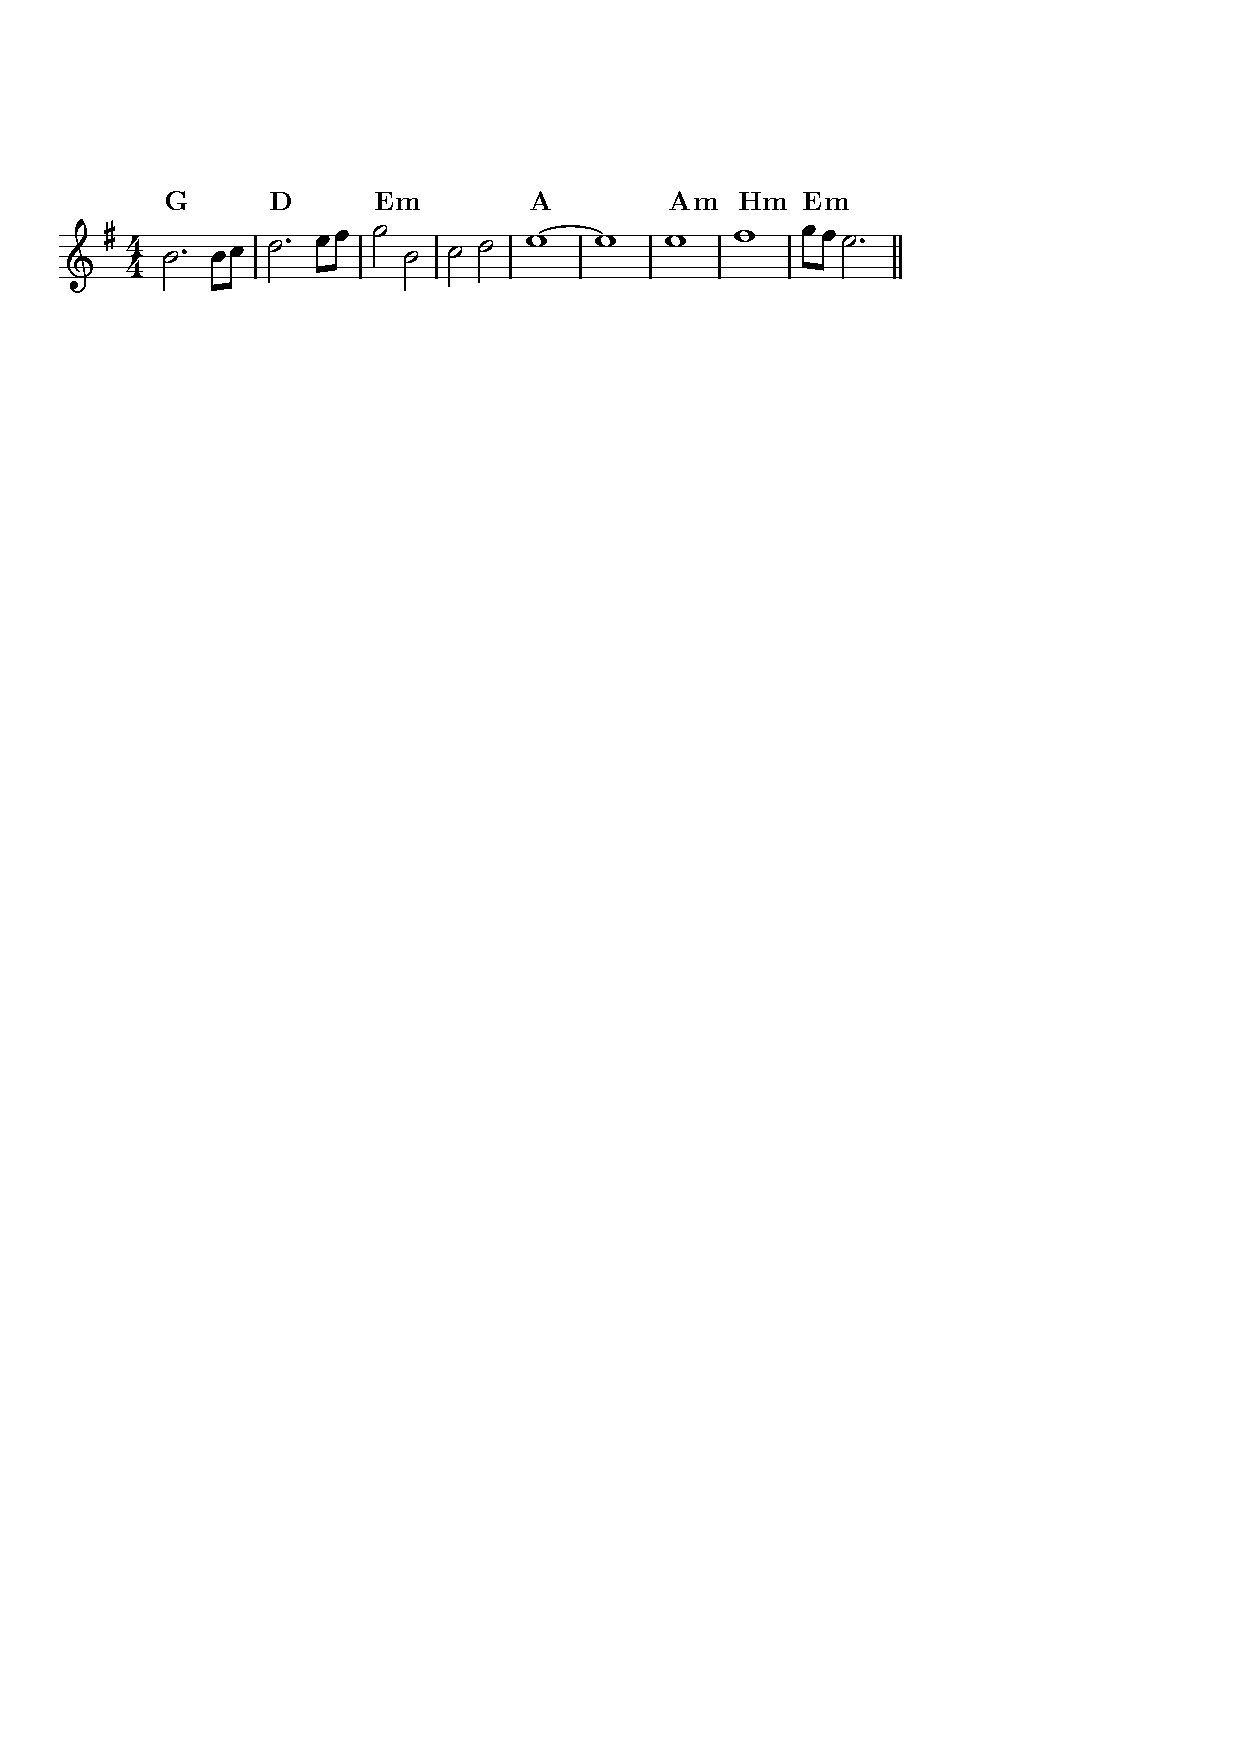
\includegraphics[width=450pt]{scores/variacenarenesancnitema.pdf}\\
\textbf{Em Em\7 Em\6 Em Em\7 Em\6}
}

\vers{2}{
Láska je jako krásná loď, která ztratila kapitána,\\
námořníkům se třesou ruce a bojí se, co bude zrána.\\
Láska je jako bolest z probuzení a horké ruce hvězd,\\
které ti oknem do vězení květiny sypou ze svatebních cest,\\
které ti oknem do vězení květiny sypou ze svatebních cest.
} \refsm{}

\vers{3}{
Láska je jako večernice plující černou oblohou,\\
náš život hoří jako svíce a mrtví milovat nemohou,\\
náš život hoří jako svíce a mrtví milovat nemohou.
} \refsm{}
\newpage
